%%「論文」,「レター」,「レター(C分冊)」,「技術研究報告」などのテンプレート
%% v3.2 [2019/03/19]
%% 4. 「技術研究報告」
\documentclass[technicalreport]{ieicej}
\usepackage[dvips]{graphicx}
\usepackage[dvipdfmx]{graphicx,xcolor}
\usepackage[T1]{fontenc}
\usepackage{lmodern}
\usepackage{textcomp}
\usepackage{latexsym}
\usepackage[fleqn]{amsmath}
\usepackage{amssymb}

\jtitle{イジング計算機での利用に向けた$l$1ノルムのQUBO形式について}
\jsubtitle{}
\etitle{QUBO formulation of l1-norm for Ising-type computers}
\esubtitle{}
\authorlist{%
  \authorentry[]{横田 知大}{Tomohiro Yokota}{Univ}
  \authorentry[]{此島 真喜子}{Makiko Konoshima}{FUJI}
  \authorentry[]{田村 泰孝}{Tamura Hirotaka}{FUJI}
  \authorentry[]{大久保 潤}{Jun Ohkubo}{Univ,JST}}
% \authorentry[メールアドレス]{和文著者名}{英文著者名}{所属ラベル}
\affiliate[Univ]{埼玉大学 大学院理工学研究科}{Saitama university, Graduate school of science and engineering}
\affiliate[FUJI]{株式会社富士通研究所}{FUJITSU LABORATORIES LTD}
\affiliate[JST]{国立研究開発法人 科学技術振興機構}{Japan Science and Technology Agency}
%\affiliate[所属ラベル]{和文勤務先\\ 連絡先住所}{英文勤務先\\ 英文連絡先住所}

\begin{document}

\begin{jabstract}
  量子アニーリングを含むイジングモデルを用いたアニーリング法においてスパース推定を可能にするために,近年,Rectified Linear Unit(ReLU)型関数のQuadratic Unconstrained Binary Optimization(QUBO)形式の導出が提案され,それを組み合わせて$l$1ノルムのQUBO形式の導出と数値実験が行われた.
  その後,発表者らにより,$l1$ノルムの直接的なQUBO形式の導出と定式化の見直しによる,より簡略化された$l$1ノルムのQUBO形式の導出が提案された.
  しかしながら簡略化された$l$1ノルムのQUBO形式を用いたスパース推定の数値的な検証はまだおこなわれていない.
  そこで,本稿では$l$1ノルムの直接的なQUBO形式の導出法を紹介し,連続値を用いたアニーリングによる数値実験でスパース性の検証を行う.
  数値実験では,スパースな推定がされていることを確認した.
\end{jabstract}
\begin{jkeyword}
$l$1ノルム,QUBO,Legendre変換,Wolfeの双対定理
\end{jkeyword}
\begin{eabstract}
英文アブストラクト
\end{eabstract}
\begin{ekeyword}
$l$1-norm,QUBO,Legendre transformation,Wolfe duality theorem
\end{ekeyword}
\maketitle

\section{まえがき}
最適化問題の近似解を得ることに特化したアニーリングマシンが開発,提供されており,代表的なものにカナダのD-Wave.Inc\cite{d-wave01}\cite{d-wave02}の"D-Wave 2000"や富士通\cite{Digital_annealer}の"Digital Annealer",日立の"CMOSアニーリングマシン"などがある.
最適化問題は,データマイニングや機械学習などの多くの分野で利用されている.
特に,KadowakiとNishimoriによって提案された量子アニーリング法\cite{Quantum_annealing}や,同様の考え方を持つ断熱量子計算\cite{AQC}の考え方が注目を集めた.
また,これらを考え方を利用する上で問題としてシステムサイズの小ささが当時挙げられていたが,利用可能な量子ビット数が年々増加しているため,大きな最適化問題にも取り組めるようになった.

アニーリングマシンのハードウェアは入力としてQUBO形式を受け付ける.
そこで,最適化問題をQUBO形式に再定式化する必要がある.
連続変数については二進数展開を行うことでイジングタイプの変数に変換することができるが,関数の系統的な導出方法はまだ示されていない.
そのため問題をQUBO形式に置き換える研究は数多く行われている.
例えば,論理ゲートを含むいくつかのNP問題に対してはLucasによって再定式化がなされている\cite{logic_gate}\cite{formulation}.
近年では,ラベルノイズに対してロバスト性を持つ$q$-loss関数のQUBO形式の導出にLegendre変換が用いられた\cite{q-loss_formulation}.
その後,ReLU型関数のQUBO形式の導出\cite{ReLU_function}にはLegendre変換だけでは不十分であることが明らかになり,新たにWolfeの双対定理\cite{Wolfe_duality}が用いられた.
また,再定式化されたReLU型関数を組み合わせることで$l$1ノルムのQUBO形式の表現と数値実験が行われ,スパース制約にも利用できることが確認された\cite{ReLU_simmulate}.

直接的な$l$1ノルムのQUBO形式の導出と定式化の見直しによる必要変数の削減\cite{l1-norm}が発表者らによって行われたが,スパース制約の数値的な検証はまだ行われていない.
そこで本稿では,まず$l$1ノルムのQUBO形式の直接的な導出と定式化の見直しを紹介する.
そして導出したQUBO形式を用いてLASSOの再現を行い,推定結果にスパース性が現れるか検証する.

\section{$l$1ノルムとスパース推定}
スパース推定とは,多くのパラメータのうちほとんどが0で,ごく一部のみ非0の値をとるように推定する方法である.
スパース性を持つ推定方法の代表的なものにLeast Absolute Shrinkage and Selection Operator(LASSO)がある.
LASSOでは次の式をコスト関数としてもち,コストが最小となるような回帰係数ベクトル$\beta$を推定する.
\begin{eqnarray}
  S_{\lambda}(\beta)=\frac{1}{2n}\|y-X\beta\|^{2}_{2}+\lambda\|\beta\|_{1} \label{lasso_function}
\end{eqnarray}
$y\in\mathbb{R}^{n}$は観測ベクトル,$X\in\mathbb{R}^{n\times p}$は計画行列,$\beta\in\mathbb{R}^{p}$は回帰係数ベクトル,$\lambda >0$は正則化パラメータである.
$\lambda$によってスパース性の強さを調節することができる.
LASSOのコスト関数は最小二乗法のコスト関数に$l$1ノルムを加えた単純な形であり,最小二乗法と比較して,汎化性能が高く過学習を抑え,推定結果にスパース性を与えられることから機械学習でよく用いられる.

\section{QUBO形式}
アニーリングマシンはQUBO形式がハードウェアとして実装されている.QUBO形式は次のように表される.
\begin{eqnarray}
  \mathcal{H} = -\sum_{i,j}{J_{ij}\sigma_{i}\sigma_{j}}-\sum_{i}{h_{i}\sigma_{i}}. \label{QUBO_model}
\end{eqnarray}
$\sigma_{i}\in\{ 0,1\}$は$i$番目のスピンを表すスピン変数,$J_{ij}\in\mathbb{R}$は$i$と$j$のスピン間の二体相互作用,$h_{i}\in\mathbb{R}$は$i$番目のスピンに対する一体相互作用である.

このQUBO形式はコスト関数に対応しているので,最適化問題のコスト関数をQUBO形式で表現できれば,アニーリングマシンを用いて解くことができるようになる.

\section{$q$-loss関数のQUBO形式での導出}
Denchevらによって提案された$q$-loss関数とQUBO形式での導出について紹介する.
$q$-loss関数のコスト関数は次のように表され,グラフの概形は図\ref{fig:q-loss}のようになる.
\begin{figure}[t]
  \begin{center}
    \vspace{-20mm}
    \includegraphics[keepaspectratio, scale=0.3]{q-loss.pdf}
    \vspace{-20mm}
    \caption{$q=-2$の場合の$q$-loss関数}
    \label{fig:q-loss}
  \end{center}
\end{figure}
\begin{eqnarray}
  L_{q}(m)=\min{\left((1-q)^{2},(\max{(0,1-m)})^{2}\right)}. \label{q-loss_cost_function}
\end{eqnarray}
$q\in [-\infty ,0)$はパラメータであり,区間$(-q,1)$は二次関数,それ以外の区間は定数となる.
文献\cite{q-loss_formulation}において,$q$-loss関数をコスト関数のペナルティ項として用いることで,識別境界から大きく離れた外れ値に対して,ペナルティを一定にすることでロバスト性を確保できることを解説している.
また,アニーリングマシンへの実装のために,Legendre変換を用いたQUBO形式への導出も紹介されている.

\subsection{Legendre変換}
関数$f_{L}(m)$に対するLengedre変換は次のように表される.
\begin{eqnarray}
  f^{*}_{L}(\eta)&=&\sup_{m}{\{\eta m-f_{L}(m)\}} \nonumber \\
  &=& -\inf_{m}{\{f_{L}(\eta)-\eta m\}}.
\end{eqnarray}
$f^{*}_{L}$を$f_{L}$の共役関数と呼ぶ.また,関数$f_{L}$に凸性を持つ場合,任意の$x_{1},x_{2}\in\mathbb{R}$と$0<\lambda <1$について常に次の関係が成り立つ.
\begin{eqnarray}
  f_{L}(\lambda x_{1}+(1-\lambda)x_{2})\leq\lambda f_{L}(x_{1})+(1-\lambda)f_{L}(x_{2}).
\end{eqnarray}
また,$f_{L}$に対してLegendre変換を2回適用した関数$f^{**}_{L}$は元の関数$f_{L}$と一致する.

\subsection{$q$-loss関数へのLegendre変換の適用}
$q$-loss関数に対してLegendre変換などを適用することで次のQUBO形式が得られる.
\begin{eqnarray}
  L_{q}(m)=\min_{t}{\left\{(m-t)^{2}+(1-q)^{2}\frac{1-\textrm{sign}(t-1)}{2}\right\}}. \label{q-loss_QUBO_model}
\end{eqnarray}
式\ref{q-loss_QUBO_model}は$m,t$について二次形式であり,最小化の形で表現されている.
また,$m,t$は連続変数であるが,二進数展開を用いることで二体相互作用で表現可能でり,sign関数についても二進数展開時に一体相互作用として表現できる.

\section{$l$1ノルムの素朴なQUBO形式での導出}
文献\cite{l1-norm}では$l$1ノルムのQUBO形式の素朴な導出と再定式化が行われた.本章ではその導出と再定式化を紹介する.
$l$1ノルムは次のように表され,グラフの概形は図\ref{fig:l1-norm}のようになる.
\begin{figure}[t]
  \begin{center}
    \vspace{-20mm}
    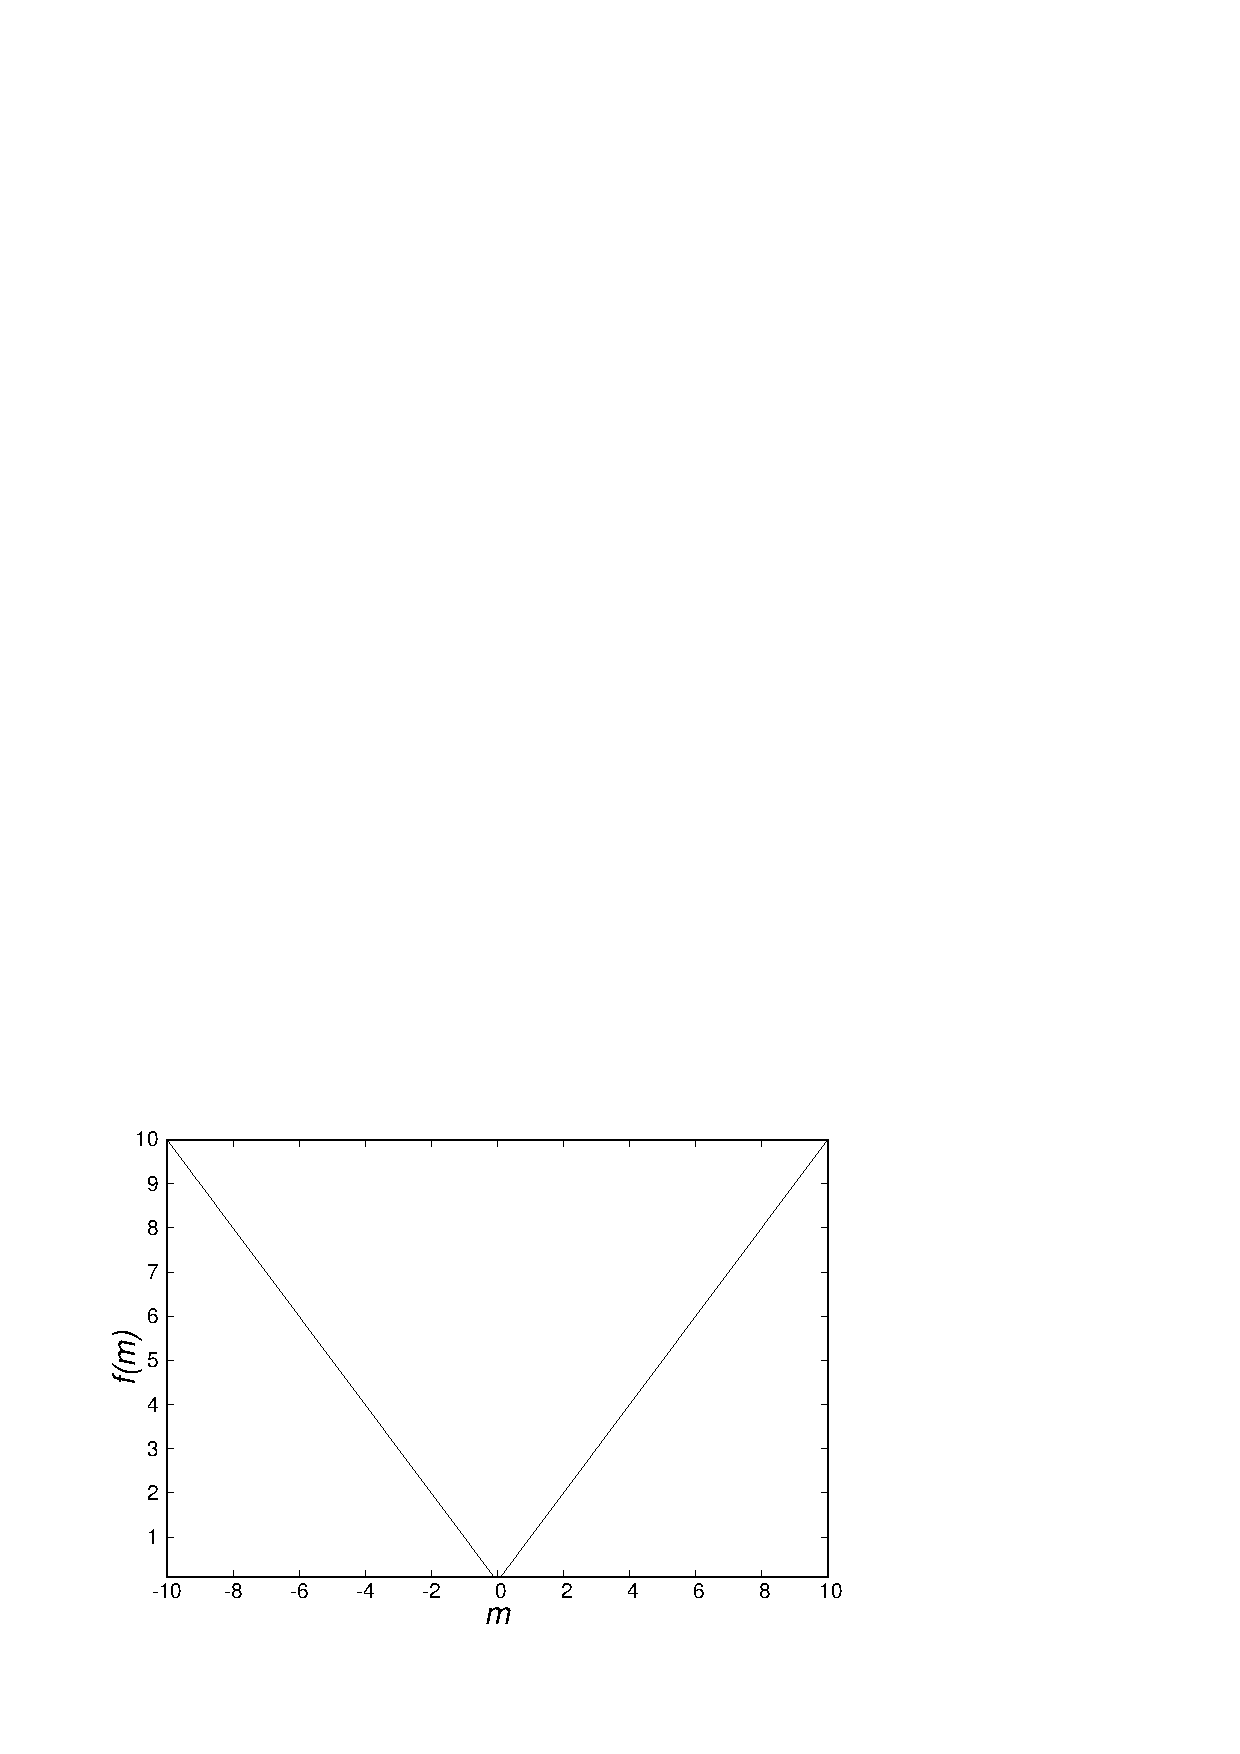
\includegraphics[keepaspectratio, scale=0.3]{absolute.pdf}
    \vspace{-20mm}
    \caption{$l$1ノルム}
    \label{fig:l1-norm}
  \end{center}
\end{figure}
\begin{eqnarray}
  f(m) = \|m\|_{1} = -\min{(-m,m)}. \label{l1-norm_01}
\end{eqnarray}
$l$1ノルムはコスト関数の正則化項としてよく用いられ,解にスパース性を与えることができる.
式\ref{l1-norm_01}にLegendre変換を適用すると二次形式は次のようになる.
\begin{eqnarray}
  F(m) = -\min_{t}{\{-mt\}} \quad (-1\leq t\leq 1). \label{l1-norm_02}
\end{eqnarray}
$f(m)$の二次形式であることを強調するために,$F(m)$とおく.

式\ref{l1-norm_02}のように,$f(m)$を二次形式で表現できたが,式\ref{l1-norm_02}では$\min$関数にマイナス符号が付いているため,$F(m)$と他のコスト関数$C(m)$を組み合わせた最適化問題を解くことできない.
\begin{eqnarray}
  \min_{m}{\left\{C(m)+F(m)\right\}} &=& \min_{m}{\left\{C(m)-\min_{t}{\left\{-mt\right\}}\right\}} \nonumber \\
  & \neq & \min_{m,t}{\left\{C(m)-(-mt)\right\}}.
\end{eqnarray}
そこで,新たにWolfeの双対定理が利用された.

\subsection{Wolfeの双対定理} \label{sec:wolfe}
Wolfeの双対定理は,次のような不等式制約付き最適化問題の双対問題の導出に用いられる.
\begin{equation}
  \left\{
  \begin{array}{lll}
    $minimize$_{x} & f_{W}(x) & (x\in\mathbb{R}^{n}), \\
    $subject to$ & h_{i}(x)\leq 0 & (i=1,2,\cdots,l). \label{wolfe_01}
  \end{array}
  \right.
\end{equation}
$f_{W}(x)$は最適化したい凸関数で,$h_{i}$は凸な不等式制約である.
目的関数と制約条件がどちらも微分可能であるとき,最適化問題に対するラグランジュ関数は次のようになる.
\begin{eqnarray}
  L(x,z) = f_{W}(x)+z^{T}h(x).
\end{eqnarray}
$z\in\mathbb{R}^{l}$はラグランジュ乗数である.Wolfeの双対定理より,式\ref{wolfe_01}の双対問題は次のように表される.
\begin{equation}
  \left\{
  \begin{array}{lll}
    $maximize$_{x,z} & L(x,z) & ((x,z)\in\mathbb{R}^{n}\times\mathbb{R}^{l}), \\
    $subject to$ & \triangledown L(x,z)=0 & (z\geq 0). \label{wolfe_02}
  \end{array}
  \right.
\end{equation}

\subsection{$l$1ノルムへのWolfeの双対定理の適用}
\ref{sec:wolfe}節で紹介したWolfeの双対定理を式\ref{l1-norm_02}に適用することで最適化問題を最大化問題に変換する.まず,式(\ref{l1-norm_02})を式(\ref{wolfe_01})の形式に書き換える.
\begin{equation}
  \left\{
  \begin{array}{ll}
    $minimize$_{t} & -mt, \\
    $subject to$ & -(t+1)\leq 0,\ t-1\leq 0. \label{l1-norm_03}
  \end{array}
  \right.
\end{equation}
Wolfeの双対定理を用いて最適化問題(\ref{l1-norm_03})の双対問題を求めると次のようになる.
\begin{equation}
  \left\{
  \begin{array}{ll}
    $maximize$_{t,z} & -mt-z_{1}(t+1)+z_{2}(t-1), \\
    $subject to$ & -m-z_{1}+z_{2}=0,\ z_{1}\geq 0,\ z_{2}\geq 0. \label{l1-norm_04}
  \end{array}
  \right.
\end{equation}

最適化問題(\ref{l1-norm_04})をQUBO形式にするためには,目的関数と制約条件を1つの式にまとめる必要がある.制約条件$-m-z_{1}+z_{2}=0$については,目的関数に次のペナルティ項を加えることで消去できる.
\begin{eqnarray}
  -M(-m-z_{1}+z_{2})^{2}. \label{penalty}
\end{eqnarray}
$M$は非常に大きな正の定数である.残りの制約条件$-1\leq t\leq 1,z_{1}\geq 0,z_{2}\geq 0$については,それぞれの制約条件の区間に一致するように二進数展開することで,QUBO形式にすることができる.

したがって,$l$1ノルムのQUBO形式は次のようになる.
\begin{eqnarray}
  &F&(m) \nonumber \\
  &=& -\min_{t}{\{-mt\}} \nonumber \\
  &=& -\max_{t,z_{1},z_{2}}{\{-mt-z_{1}(t+1)+z_{2}(t-1)} \nonumber \\
  & & \mbox{}-M(-m-z_{1}+z_{2})^{2}\} \nonumber \\
  &=& \min_{t,z_{1},z_{2}}{\{mt+z_{1}(t+1)-z_{2}(t-1)} \nonumber \\
  & & \mbox{}+M(-m-z_{1}+z_{2})^{2}\} \label{l1-norm_befor}
\end{eqnarray}

\section{余分な変数の削除}
この章では,式(\ref{l1-norm_befor})の再定式化をすることで,追加変数の削減を行う.

制約条件の1つである$-m-z_{1}+z_{2}=0$は,式(\ref{penalty})をペナルティ項として加えることで解消した.そこで,$z_{2}=m+z_{1}$を用いて式(\ref{l1-norm_befor})を次のように式変形できる.
\begin{eqnarray}
  &F&(m) \nonumber \\
  &=& \min_{t,z_{1},z_{2}}{\{mt+z_{1}(t+1)-z_{2}(t-1)} \nonumber \\
  & & \mbox{}+M(-m-z_{1}+z_{2})^{2}\} \nonumber \\
  &=& \min_{t,z_{1},z_{2}}{\{mt+z_{1}(t+1)-(m+z_{1})(t-1)} \nonumber \\
  & & \mbox{}+M(-m-z_{1}+z_{2})^{2}\} \nonumber \\
  &=& \min_{z_{1},z_{2}}{\{z_{1}+(m+z_{1})+M(-m-z_{1}+z_{2})^{2}\}} \nonumber \\
  &=& \min_{z_{1},z_{2}}{\{z_{1}+z_{2}+M(-m-z_{1}+z_{2})^{2}\}} \label{l1-norm_after}
\end{eqnarray}
論文\cite{l1-norm}では連続値を用いた数値実験で式(\ref{l1-norm_after})が$l$1ノルムを表現していることを確認した.

\section{スパース推定への適用}
この章では式(\ref{l1-norm_after})を用いてスパース推定を行う.LASSOのコスト関数である式(\ref{lasso_function})は式(\ref{l1-norm_after})を用いて次のように表せる.
\begin{eqnarray}
  S_{\lambda}(\beta) &=& \|y-X\beta\|^{2}_{2} \nonumber \\
  & & \mbox{}+\lambda\sum^{p}_{i=1}{\min_{z_{1i},z_{2i}}{\{z_{1}+z_{2}+M(-\beta_{i}-z_{1i}+z_{2i})^{2}\}}} \nonumber \\
  \label{lasso_function_01}
\end{eqnarray}

以降の節では,数値実験で利用したデータセットと実験の詳細についての説明,および実験の結果をまとめる.

\subsection{人工データセット}
実験で利用するデータセット$X$は,データ数が$500$,次元数が$5$でガウス分布$\mathcal{N}(0,1)$に従うものとする.また,解にあたる回帰係数ベクトル$\beta$は推定結果がスパースになるかの検証を行いやすくするために,一様乱数$\mathcal{U}(-10,10)$とし,ノイズ$\epsilon$を$\mathcal{N}(0,0.1)$のように設定した.これらを用いて観測ベクトル$y$を次のようにとる.
\begin{eqnarray}
  y = X\beta +\epsilon
\end{eqnarray}

\subsection{座標降下法}

\subsection{実験方法の詳細}
本節では式(\ref{lasso_function_01})のQUBO形式が適切に機能することでスパースな推定が行われるかをシミュレーテッドアニーリングを用いて検証し,座標降下法での推定結果と比較する.シミュレーテッドアニーリングのアルゴリズムとしてメトロポリス法を用いる.メトロポリス法のアルゴリズムは次のようになる.
\begin{enumerate}
\item[(1)] 初期状態を$0$とする.
\item[(2)] 現在の状態を$x$とし,次の状態$x'$を確率的に選ぶ.
\item[(3)] 候補の状態$x'$のエネルギー$E'$の現在の状態$x$のエネ\\
  $\qquad \quad \ $ ルギー$E$の差分$\Delta E=E'-E$を計算する.
\item[(4)] $\Delta E<0$:確率$1$で候補$x'$を受理する.\\
  $\qquad \quad \ \ \Delta E\geq 0$:確率$-\exp (\Delta E/T)$で候補$x'$を受理する.
\item[(5)] 温度$T$を下げる.
\item[(6)] $(2)$から$(5)$の処理を繰り返す.
\end{enumerate}
温度$T$の冷却スケジュールには次の式を用いる.
\begin{eqnarray}
  T_{k+1} = \alpha T_{k}
\end{eqnarray}
$k$は現在のステップ数であり,$0<\alpha <1$である.本実験では変数を二進数展開せずに連続値を用いた.また,各変数の遷移については次のように設定した.
\begin{eqnarray}
  \beta_{k+1} = \beta_{k} + \epsilon \\
  z_{k+1} = z_{k} + \epsilon ' \quad (z<0のときz=0)
\end{eqnarray}
$\epsilon\sim\mathcal{N}(0,\sigma_{k}),\epsilon '\sim\mathcal{N}(-\frac{1}{4}\sigma_{k},\sigma_{k})$で次の状態へ遷移する.また,$\sigma_{k}$は遷移距離であり,スケジュールには次の式を用いる.
\begin{eqnarray}
  \sigma_{k+1} = \alpha \sigma_{k}
\end{eqnarray}
$z$が負の方向へ遷移しやすく設定したのは,論文\cite{l1-norm}で式(\ref{l1-norm_after})が最適値を取るとき,各変数が次の値に収束するためである.
\begin{itemize}
\item $m\geq 0$の場合:$z_{1}=0,\quad z_{2}=m$
\item $m<0$の場合:$z_{1}=-m,\ z_{2}=0$
\end{itemize}

\subsection{実験の結果}
アニーリングの設定は,初期温度$T_{0}=50$,$t=5,000,000$,$\sigma_{0}=1$,$\alpha=0.999999$を用いた.$\lambda =\{1,2,4\}$に対する線形回帰の結果の比較を表\ref{table:result}に示す.左は解を表し,各$\lambda$に対するシミュレーテッドアニーリングと座標降下法との推定結果である.
\begin{table}[b]
  \begin{center}
    \caption{CDとSAでの推定結果の比較}
    \label{table:result}
    \begin{tabular}{|c||c|r|r|r|r|r|r|} \hline
      & 解($\beta$) & \multicolumn{2}{|c|}{$\lambda =1$} & \multicolumn{2}{|c|}{$\lambda =2n$} & \multicolumn{2}{|c|}{$\lambda =4n$} \\ \hline \hline
      & & CD & SA & CD & SA & CD & SA  \\ \hline
      $\beta_{1}$ &  0.32797 &  0.33 &  0.33 &  0.00 &  0.00 &  0.00 &  0.00 \\
      $\beta_{2}$ &  1.05080 &  1.04 &  1.04 &  0.10 &  0.10 &  0.00 &  0.00 \\
      $\beta_{3}$ &  1.41335 &  1.35 &  1.36 &  0.26 &  0.26 &  0.00 &  0.00 \\
      $\beta_{4}$ &  9.05368 &  8.87 &  8.91 &  7.84 &  7.87 &  6.82 &  6.85 \\
      $\beta_{5}$ & -9.43051 & -9.07 & -9.10 & -8.16 & -8.19 & -7.16 & -7.19 \\ \hline
    \end{tabular}
  \end{center}
\end{table}
  
  
%\bibliographystyle{sieicej}
%\bibliography{myrefs}
\begin{thebibliography}{99}% 文献数が10未満の時 {9}
\bibitem{d-wave01}
  M.W.Johnson, M.H.S. Amin, S. Gildert, T.Lanting, F. Hamze, N.Dickson, R. Harris, A.J. Berkley, J. Johansson, P. Bunyk, E.M. Chapple, C. Enderud, J.P. Hilton, K. Karimi, E. Ladizinsky, N. Ladizinsky, T. Oh, I. Perminov, C. Rich, M.C. Thom, E. Tolkacheva, C.J.S. Truncik, S. Uchikin, J. Wang, B. Wilson and G. Rose, "Quantum annealing with manufactured spins," Nature vol.473, pp.194-198, May 2011.
  
  DOI:10.1038/nature10012
\bibitem{d-wave02}
  P.I. Bunyk, E. Hoskinson, M.W. Johnson, E. Tolkacheva, F. Altomare, A.J. Berkley, R. Harris, J.P. Hilton, T. Lanting, A.J. Przybysz and J. Whittaker, "Architectural Considerations in the Design of a Superconducting Quantum Annealing Processor," Proc. IEEE, vol.24, no.4, August 2014.
  
  DOI:10.1109/TASC.2014.2318294
\bibitem{Digital_annealer}
  M. Aramon, G. Rosenberg, E. Valiante, T. Miyazawa, H. Tamura and H.G. Katzgraber, "Physics-Inspired Optimization for Quadratic Unconstrained Problems Using a Digital Annealer," Front. Physics 7:48. Mar 2019.
  
  DOI:10.3389/fphy.2019.00048
\bibitem{Quantum_annealing}
  T. Kadowaki and H. Nishimori, "Quantum annealing in the transverse Ising model," Phys. Rev. E, vol.58, Nov 1998.
  
  DOI:10.1103/PhysRevE.58.5355
\bibitem{AQC}
  E. Farhi, J. Goldstone, S. Gutmann, J. Lapan, A. Lundgren and D. Preda, "A quantum adiabatic evolution algorithm applied to random instances of an NP-complete problem,"
\bibitem{formulation}
  A. Lucas, "Ising formulations of many NP problems," Front. Physics 2:5. Feb 2014.
  
  DOI:10.3389/fphy.2014.00005
\bibitem{logic_gate}
  J.D. Whitfield, M. Faccin and J.D. Biamonte, "Ground-state spin logic," EPL, vol.99, Sept 2012.
  
  DOI:10.1209/0295-5075/99/57004
\bibitem{q-loss_formulation}
  V. Denchev, N. Ding, S.V.N. Vishwanathan, and H. Neven, "Robust Classification with Adiabatic Quantum Optimization," Proc. 29th International Conf. on Machine Learning, pp.863-870, Jul 2012.
\bibitem{ReLU_function}
  G. Sato, M. Konoshima, T. Ohwa, H. Tamura, and J. Ohkubo, "Quadratic unconstrained binary optimization formulation for rectified-linear-unit-type function," Phys. Rev. E, vol.99, Apr 2019.
\end{thebibliography}

\end{document}
